%
% First comes an example EPS file -- just ignore it and
% proceed on the \documentclass line
% your LaTeX will extract the file if required
\begin{filecontents*}{example.eps}
%!PS-Adobe-3.0 EPSF-3.0
%%BoundingBox: 19 19 221 221
%%CreationDate: Mon Sep 29 1997
%%Creator: programmed by hand (JK)
%%EndComments
gsave
newpath
  20 20 moveto
  20 220 lineto
  220 220 lineto
  220 20 lineto
closepath
2 setlinewidth
gsave
  .4 setgray fill
grestore
stroke
grestore
\end{filecontents*}
%
\RequirePackage{fix-cm}
%
% \documentclass{svjour3}                     % onecolumn (standard format)
%\documentclass[smallcondensed]{svjour3}     % onecolumn (ditto)
\documentclass[smallextended]{svjour3}       % onecolumn (second format)
%\documentclass[twocolumn]{svjour3}          % twocolumn
%
\smartqed  % flush right qed marks, e.g. at end of proof
%
\usepackage{graphicx}
\usepackage[most]{tcolorbox}
\usepackage{listings}
\usepackage{xcolor}
\usepackage{subcaption}
\usepackage{tabularx}
\usepackage{booktabs}
\usepackage[colorinlistoftodos,prependcaption,textsize=tiny]{todonotes}
\usepackage{wrapfig}

\definecolor{backcolor}{rgb}{0.95,0.95,0.92}
\colorlet{punct}{red!60!black}
\definecolor{delim}{RGB}{20,105,176}
\colorlet{numb}{magenta!60!black}

\lstdefinestyle{mystyle}{
  language=Python,
  basicstyle=\ttfamily\footnotesize,
  keywordstyle=\color{delim},
  stringstyle=\color{punct},
  commentstyle=\color{numb},
  breakatwhitespace=true,
  breaklines=true,
  keepspaces=true,
  showspaces=false,
  showstringspaces=false,
  showtabs=false,
  tabsize=2,
  stepnumber=1,
  numbersep=3pt,
  captionpos=b,
  numbers=left,
  numberstyle=\tiny\color{gray},
  backgroundcolor=\color{backcolor},
  aboveskip=0pt,
  belowskip=0pt
}
\lstset{style=mystyle}

\lstset{emph={%  
    assert%
    },emphstyle={\color{delim}}%
}%

%
% \usepackage{mathptmx}      % use Times fonts if available on your TeX system
%
% insert here the call for the packages your document requires
%\usepackage{latexsym}
% etc.
%
% please place your own definitions here and don't use \def but
% \newcommand{}{}
%
% Insert the name of "your journal" with
% \journalname{myjournal}
%
\begin{document}

\title{Exploring the Role of Feedback in Machine Learning Jupyter Notebooks}

%\titlerunning{Short form of title}        % if too long for running head

\author{Arumoy Shome\and
  Lu{\`\i}s Cruz\and
  Diomidis Spinellis\and
  Arie van Deursen
}

%\authorrunning{Short form of author list} % if too long for running head

\institute{A. Shome \at
  Delft University of Technology\\
  \email{a.shome@tudelft.nl}
  \and
  L. Cruz \at
  Delft University of Technology\\
  \email{l.cruz@tudelft.nl}
  \and
  D. Spinellis \at
  Delft University of Technology\\
  \email{d.spinellis@tudelft.nl}
  \and
  A. V. Deursen \at
  Delft University of Technology\\
  \email{arie.vandeursen@tudelft.nl}
}

\date{Received: date / Accepted: date}
% The correct dates will be entered by the editor


\maketitle

\begin{abstract}

  \todo{update the numbers here}
Testing ML systems is a highly interactive process which demands a human-in-the-loop approach. In addition to writing tests for the code base, practitioners are required to analyse and interpret several visualisations using their domain expertise to validate if an ML system satisfies the required set of functional and non-functional properties. Visualisations are frequently used to qualitatively assess various parts of an ML pipeline. However, implicit knowledge gained from visualisations must be translated to explicit analytical tests that fail when there is change in any component of the ML pipeline. We conduct an empirical analysis of Jupyter notebooks to catalogue the state-of-the-art mappings between ML visualisations and assertions. We mine Github to collect 54K Jupyter Notebooks that contain assertions written in Python. We develop a novel methodology to identify 1764 notebooks which contain an assertion below a visualisation. We manually analyse the 1.7K notebooks and identify 269 visualisation-assertion pairs that are semantically related to one another. We further investigate the 269 visualisation-assertion pairs and identify three frequently occurring testing patterns. We perform an in-depth analysis of 34 visualisation-assertion pairs and find that the assertions often fail to capture all the information present in their visual counter-part. Empirical evidence obtained in this study indicates that current software testing methods fail to address the unique challenges of ML. And emphasises the need for automated tools that bridge the gap between visual assessments and analytical assertions.

\keywords{ML Testing \and SE4AI \and Visualisations \and Assertions \and Computational Notebooks}
\end{abstract}

\section{Introduction}

% amershi2019software: start with ML development life cycle and how everything is done in a very iterative way; things are dependant on one another; etc.

% martinez-plumed2021crisp-dm: not only does ML include the crip-dm framework, but this same form of iteration is seen in the model development and experimentation phase;

% this is why we see the use of computational notebooks being widely adopted by the ML community

% writing ML code is more iterative and requires a constant feedback; we identify this feedback can be provided in two ways: implicitly from the output of a cell and explicitly from a failed assertion

Code, data and ML model in ML-enalbed systems are highly tangled with each other. For instance, the decision to use a particular type of ML model, requires a deep understanding of the data which will be used to train the model. Data quantity and quality directly influence the complexity of the ML model. 

Conversely, the choice of the ML model also influences the data pre-processing and transformation steps that are required to get the data ready for training. For instance, using a classic statistical model requires several data transformation steps such as scaling and normalization, and converting categorical features to numerical ones using one-hot encoding.

Visualisations are used throughout the ml development lifecycle to test various properties of the ml system. in the early stages of the ml development lifecycle, visualisations are extensively used to make sense of the data and verify its statistical properties. during the model development phase, visualisations are used to summarise metrics, contrast different learning algorithms and iteratively fine-tune ml models. once the model is deployed in production, visualisations are used to continually monitor their performance and trigger a new training cycle once their performance drops below a certain threshold~\cite{yuan2021survey,hohman2019visual,amershi2015modeltracker,wexler2020if}.

building ml systems is highly iterative and experimental. information gained from ml visualisations is used to make design and implementation decisions for the following steps of the ml pipeline. for instance, we may visualise the distribution of our training data and find that it is normally distributed. based on this information, we may opt for a linear regression model which assumes normality in the underlying data. however, such expectations regarding the data may be violated once the ml system is deployed in production, where the data constantly changes as a reflect of the real world~\cite{amershi2019software,sambasivan2021everyone,breck2019data,baylor2017tfx}.

implicit expectations obtained from visualisations must therefore be
translated to analytical tests that fail once our expectations
regarding the ml system are no longer satisfied.

in contrast to prior work, we approach ml testing from a new
perspective. we conduct an empirical analysis of computational
notebooks obtained from github, to understand the process of testing
ml systems in practice. in particular, we focus on the combination of
a qualitative form of testing (using visualisations) and a
quantitative form of testing (using analytical assertions). the
research questions along with the contributions of this paper are as
follows.

\begin{description}
  \item[rq1.] \textbf{how frequently are analytical tests formulated
    from visualisations created to test ml systems?}

    we mine 54k jupyter notebooks from github that contain an assertion
    written in python. we develop an automated technique to identify 1764
    notebooks with an assertion below a visualisation. we manually analyse
    the 1.7k notebooks and identify 269 visualisation-assertion (va) pairs
    that are semantically related to each other. we plan to release this
    catalogue of va pairs publicly.

\item[rq2.] \textbf{what patterns are frequently observed in va pairs
  used to test ml systems?}

  we analyse the 269 va pairs from rq1, and observe three testing
  patterns that frequently occur in the va pairs.

\item[rq3.] \textbf{do the assertions capture all the information
  obtained from the corresponding visualisation?}

  we further perform an in-depth analyse of 34 va pairs (and their
  corresponding notebooks). we observe that assertions often cannot
  capture all the information obtained from the visualisation.

\end{description}

our observations indicate that formulating analytical assertions from
visualisations is an emerging testing technique. however, the
assertions found in this study often do not reflect the information
obtained from their visual counter-part. this study finds the need for
automated tools that can reduce the manual effort necessary to
validate visualisations in ml systems. and help ml practitioners to
formulate better analytical assertions from visualisations.

the replication package for this study is made public on
figshare\footnote{the replication package can be found at this url:
https://figshare.com/s/9347228011999cba29f5}.

\section{Preliminaries}\label{sec:prelim}

This section summarises prior scientific work that has been done in ML
Testing, computational notebooks and visual analytics. The section
concludes with an overview of technical knowledge required for this
paper.

\subsection{ML Testing}\label{sec:ml-testing}

Testing ML enabled software systems poses more challenges compared to
their traditional counter part. While traditional software systems
mature through change in their codebase, ML enabled systems
additionally experience change in the training data and the machine
learning
model~\cite{sculley2015hidden,amershi2019software,sambasivan2021everyone}.
With ML being adopted into safety-critical domains that can affect
human lives, ensuring that ML systems are correct, robust to data
perturbations and not biased by race, colour or gender is of paramount
importance. Existing scientific literature on ML testing broadly
focuses on two aspects. First, on functional properties such as
correctness and robustness of the model towards unseen data. And
second, on non-functional properties such as fairness,
interpretability and
privacy~\cite{zhang2020machine,mehrabi2021survey,chen2022fairness}.

To test the correctness of ML models, several improvements over
existing test adequacy metrics have been proposed. Tools such as
\textit{DeepExplore} and \textit{DeepGauge} propose new test adequacy
metrics such as neuron coverage adapted for ML enabled software
systems~\cite{pei2017deepexplore, ma2018deepgauge,
  gerasimou2020importance}. Formal verification methods have also been
proposed that try to provide formal guarantee of robustness against
adversarial examples. Such methods however are only feasible for
statistical ML models and become computationally expensive for more
complex models such as deep neural networks~\cite{zhu2021deepmemory,
  baluta2021scalable}. Several works have been conducted on generating
and detecting adversarial inputs for ML models. Data augmentation
techniques based on fuzzing, search based software testing and
mutation testing have been proposed to generate adversarial examples
that can be used during model training to improve its
robustness~\cite{braiek2019deepevolution, gao2020fuzz, wang2021robot,
  zhang2020white}. It is however not possible to include all
variations of adversarial examples into the training data. Thus,
methods have been proposed to detect adversarial inputs during
runtime~\cite{xiao2021self, wang2020dissector, wang2019adversarial,
  berend2020cats}.

In contrast to existing scientific contributions, we conduct a
large-scale empirical analysis of Jupyter Notebooks to understand the
process of testing ML systems. Specifically, we focus on how
visualisations are used to test specific properties of ML systems. We
further investigate how frequently analytical tests are formulated
based on the information gained from the visualisations.

\subsection{Computational Notebooks and Software Engineering}\label{sec:notebooks}

Computational notebooks have been ubiquitously adopted by the machine
learning community for developing ML enabled systems. Although
originally intended to promote reproducible software, computational
notebooks are far from being reproducible due to lack of software
engineering best practices such as separation of concern, testing and
versioning~\cite{pimentel2019large,wang2020better,chattopadhyay2020wrong}.

\emph{Psallidas et al} provide an overview of the evolving landscape
of computational notebooks by analysing six million Python notebooks,
two million enterprise Data Science (DS) pipelines, source code and
metadata from over 900 releases of 12 important DS libraries. Their
findings can be used by system builders for improving DS tools and
also by DS practitioners to understand the current trends in
technologies they should focus on. \emph{Pimentel et al} mined 1.4
million notebooks from Github to conduct an empirical study on the
coding practices in computational notebooks. Based on their analysis,
the authors propose guidelines on improving reproducibility of
computational notebooks. To enable future research on computational
notebooks, \emph{Quaranta et al} mine Kaggle and present
\textit{KGTorrent}, a public dataset consisting of approximately 2.5
million Jupyter notebooks written in Python. The dataset also contains
a relational database dump of metadata regarding publicly available
notebooks on Kaggle.

Studies with human subjects have been conducted to gain a deeper
understanding of the challenges faced by ML practitioners when
developing ML models inside notebooks. The results indicate that ML
practitioners work in a highly iterative fashion, often experimenting
with multiple strategies to analyse the data or produce meaningful
visualisations~\cite{kandel2012enterprise, kery2018story,
  liu2019understanding, chattopadhyay2020wrong}. Studies have also
been conducted to understand how practitioners generate, evaluate and
manage alternative hypothesis, visual designs, methods, tools,
algorithms and data sources to arrive at the final
implementation~\cite{liu2019understanding,kandel2012enterprise}. The
findings from these studies can be used as guidelines for improving
existing notebook technologies or designing new ones.

To manage and prune multiple versions of code that accumulate over
time when developing in notebooks, \emph{Head et al} propose a code
gathering tool that allows practitioners to review and only keep the
relevant version of code. Other tools such as \textit{WrangleDoc} and
\textit{VizSmith} have also been proposed to aid ML practitioners when
working within computational notebooks~\cite{yang2021subtle,
  bavishi2021vizsmith}.

Jupyter notebooks have been widely adopted by the DS and ML
communities to develop ML
pipelines~\cite{wang2020assessing,pimentel2019large,quaranta2021kgtorrent}.
Computational notebooks provide a rich source of data in the form of
natural text, code and visualisations. Computational notebooks also
allow ML practitioners to present the knowledge gained from the
analysis in a narrative that can be shared with
others~\cite{rule2018exploration}. This study leverages the
computational narrative present within notebooks to identify
visualisations and assertions that are semantically linked to each
other.

\subsection{Visualisations and Machine Learning}\label{sec:visualisations}

As ML augment software systems in safety-critical domains, emphasis
has been put into explainability of ML models. ML models and the
underlying data is complex and multi-dimensional. To combat the
``curse of dimensionality'', visual analytics has been widely adopted
by the ML community to understand the data and the internal workings
of ML models~\cite{yuan2021survey,hohman2019visual,wexler2020if}.

Prior studies have been conducted to understand how visual analytics
techniques are currently being used in ML. \emph{Yuan et al} conduct a
systematic review of 259 papers and propose a taxonomy of visual
analytics techniques for ML. \emph{Hohman et al} conduct a survey of
visual analytics techniques for Deep Learning Models. The findings of
the study indicate that visual analytics has been widely adopted in ML
for model explanation, interpretation, debugging and improvement.

Several tools have been proposed by the visual analytics research
community to aid practitioners in understanding how their ML models
operate. \emph{Wexler et al} propose \textit{What-If}, a visual
analytics tool to explore alternative hypotheses, generate
counterfactual reasoning, investigate decision boundaries of the model
and how change in data affects the model predictions. To reduce the
cognitive load of ML practitioners during model building phase,
\emph{Amershi et al} propose \textit{ModelTracker}. Given a trained
model and a sample dataset, ModelTracker presents all the information
in traditional summary statistics along with the performance of the
model.

\textit{ESCAPE}, \textit{GAM Coach}, \textit{Angler} and
\textit{Drava} are a few other tools that have been proposed to handle
specialised use-cases such as identifying systematic errors in ML
models, generating counterfactual explanations for Generalised
Additive Models, prioritising machine translation model improvements
and relating human concepts with semantic dimensions extracted by ML
models during disentangled representation learning\cite{ahn2023escape,
  wang2023gam, robertson2023angler, wang2023drava}.

In contrast to prior work which propose dedicated visual analytics
tools, this study focuses on visualisations within computational
notebooks. We focus on visualisations produced by AI practitioners
using Python libraries (such as Matplotlib or Seaborn). Additional
context provided by surrounding code and markdown cells are used to
understand the motivation for creating the visualisation and the
information gained from it.

\section{Study Design}

\todo{TODO: introduce the motivation of the study along with the RQs here}

% role of feedback in writing ML code? (any recommendation for papers I can refer to here?)
% implicit vs. explicit feedback (how do we establish this concept?)

\subsection{Data Collection}\label{sec:data-collect}

\begin{figure}
\centering
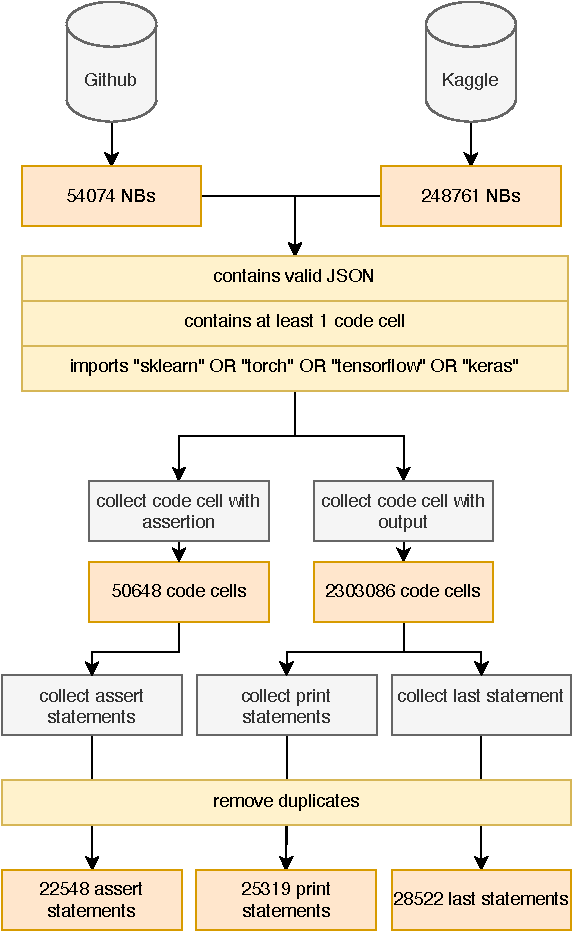
\includegraphics[width=\linewidth]{data-collection.pdf}
\label{fig:data-collection}
\caption{Overview of data collection methodology used in this study}
\end{figure}

Figure~\ref{fig:data-collection} summarises the data collection procedure used in this study. We collected Jupyter notebooks written in Python, from Kaggle and Github. 

We mined public repositories from Github to collect $49923$ Jupyter notebooks. We use the Github advanced search syntax~\footnote{https://docs.github.com/en/search-github/searching-on-github/searching-code} to isolate Jupyter Notebook that contain the keyword ``assert'' in them. The final search query is as follows: \texttt{"assert" language:"Jupyter Notebook"}.\footnote{Collected on June 22, 2023}

For Kaggle, we used a pre-existing dataset KGTorrent~\cite{quaranta2021kgtorrent} since Kaggle does not support advanced code-based search like Github. To the best of our knowledge, KGTorrent this is the largest dataset of Python Jupyter notebooks obtained from Kaggle consisting of $248763$ notebooks.

Therefore, we start with 283GB of data comprising of $298686$ Python Jupyter notebooks.

We check the validity of the underlying JSON structure in each notebook using the nbformat tool ~\footnote{https://nbformat.readthedocs.io/en/latest/}. Since the focus of this study is on the analysis of Python code, we only include notebooks that contain at least one code cell. Finally, to focus on Python code written specifically for ML projects, we only include notebooks that import popular ML libraries~\footnote{These libraries are derived from white literature---https://www.coursera.org/articles/python-machine-learning-library, https://www.geeksforgeeks.org/best-python-libraries-for-machine-learning, https://www.datacamp.com/blog/top-python-libraries-for-data-science, https://www.kdnuggets.com/2020/11/top-python-libraries-data-science-data-visualization-machine-learning.html, https://lp.jetbrains.com/python-developers-survey-2022}.

For explicit feedback using assertions, we programmatically analyse the JSON structure of the notebooks to isolate code cells. We collect Python assert statements from the code cells by constructing and subsequently parsing the Abstract Syntax Tree (AST) of the source code present in each cell.

\todo{TODO: justify why we didn't collect failures (strerr); that is more debugging? not the focus of this paper?}
Similarly, for implicit feedback, we first isolate code cells that produce an output. The output of a cell may either be from a ``print'' statement or the last statement of the cell. We collect both of them using the AST of the cell.

Finally, we remove duplicate data points (asserts, prints and last statements) resulting in a final data set of $22548$ assertions, $25319$ print statements and $28522$ last statements.

\subsection{Case Studies}

\todo{TODO: might need a visual aid here}

We allocated a fixed time resource of 100 hours to conduct the case study analysis of all candidates (assertions and cell outputs). To surface interesting candidates for the case studies, we apply NLP techniques as described below.

\todo{TODO: point out the poor quality of notebooks out there (we have citations for this); and the resulting noise in the assertions/outputs. Thats why we need to apply these tecniques to surface unique and interesting candidates!}

The assertions and cell outputs are first tokenised---special characters and alpha-numeric words shorter than two characters are removed. Two stop words namely ``assert'' and ``print'' are removed since they appear in all assertions and print statements respectively. The term frequency (TF) for all tokens is calculated and then normalised using their inter-document frequency (IDF) such that tokens thay appear less frequently are assigned a higher value.

We apply stratified random sampling to identify the candidates for the case study analysis. The sub-groups are created by adding TF-IDF of the tokens in each candidate to produce an aggregate value. The candidates are then divided into quartiles based on the aggregate value. A candidate is randomly drawn from each bin and analysed as an in-depth case study. The analysis is stopped when the time resource is exhausted.

During each case study, we analyse the code of the candidate to understand its purpose. Additionally, we analyse the entire code cell, the previous cell, next cell and the notebook's purpose to bring in rich context.

\section{Results}

\subsection{Implicit feedback from the output of code cells}

\subsubsection{Data distribution check ($N = 7$)}
% (O2, O4, O9, O14, O20, O25, O48)

\begin{table}
\centering
\caption{Examples of cell outputs used to verify distribution of data.}
\begin{tabular}{@{}m{0.05\textwidth} m{0.4\textwidth} m{0.3\textwidth}@{}}
\toprule
\emph{\textbf{Key}}&
\emph{\textbf{Code}}&
\emph{\textbf{Description}}\\
\midrule

O14&
\begin{lstlisting}
pd.pivot_table(train, index='Survived', values=['Age', 'SibSp', 'Parch', 'Fare'])
\end{lstlisting}&
Check the mean value of the specified features for each label in the target feature.\\

O48&
\begin{lstlisting}
x_train.describe()
\end{lstlisting}&
Check the descriptive statistics of the training data. The above statement is written immediately after normalising the features in the training data.\\

\bottomrule
\end{tabular}
\label{tab:distribution-check}
\end{table}

\begin{figure*}
\centering
\subcaptionbox{Check the distribution of the feature \texttt{Age} with-respect-to the labels in the target feature \texttt{Survived}.\label{fig:distribution-check-kdeplot}}{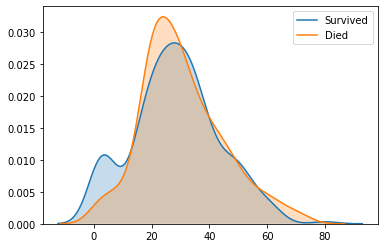
\includegraphics[width=0.45\linewidth]{distribution-check-kdeplot.png}}
\subcaptionbox{Check the distribution of the feature \texttt{likes} across all values of feature \texttt{category\_id}.\label{fig:distribution-check-catplot}}{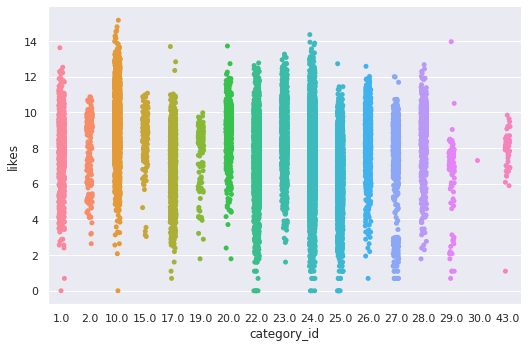
\includegraphics[width=0.45\linewidth]{distribution-check-catplot.png}}
\caption{Examples of visualisations used to check linear relationship in data.}
\label{fig:distribution-check}
\end{figure*}

Understanding the distribution of data is crucial for making informed decisions regarding necessary data transformation steps in data analysis processes. For instance, identifying whether scaling, normalizing, or handling outliers is required can be efficiently and effectively determined through visualizations.

% This is particularly important for models like linear regression, which perform optimally when data is normally distributed. If the data deviates from normality, additional transformation steps may be necessary to prepare it for training.


During the exploratory data analysis (EDA) or data understanding phase, a combination of visualizations and pandas dataframes is often employed to assess the distribution of specific columns within the data. This step helps identify features that may have a relationship with the target variable, ultimately informing which features to include in the machine learning model training process. This is seen in Figure~\ref{fig:distribution-check-kdeplot} where the distribution of a feature \texttt{Age} is checked against the labels of the target feature. Figure~\ref{fig:distribution-check-catplot} presents another example where the distribution of a continuous feature \texttt{likes} is checked with-respect-to all the values of another categorical feature \texttt{category\_id}.

For example, the distribution of a newly created feature, such as one where a continuous feature is binned into categories, is frequently examined. 

Descriptive statistics are also used post-transformation to verify that steps like data normalization have been effectively applied, ensuring that the data conforms to the expected format for further analysis.


Furthermore, distribution checks are often performed immediately after feature creation. For instance, this may occur after discretizing a continuous feature using binning. Additionally, descriptive statistics (e.g., mean and standard deviation) obtained from libraries like pandas can be used to verify the effectiveness of data normalization steps.

\subsubsection{Data relationship check ($N = 2$)}
% (O6, O10)
\todo{TODO: I think correlation checks should also be present in this group}

\begin{figure*}
\centering
\subcaptionbox{Using a lineplot to check linear relationship between two features in a dataset.\label{fig:linear-relation-check-lineplot}}{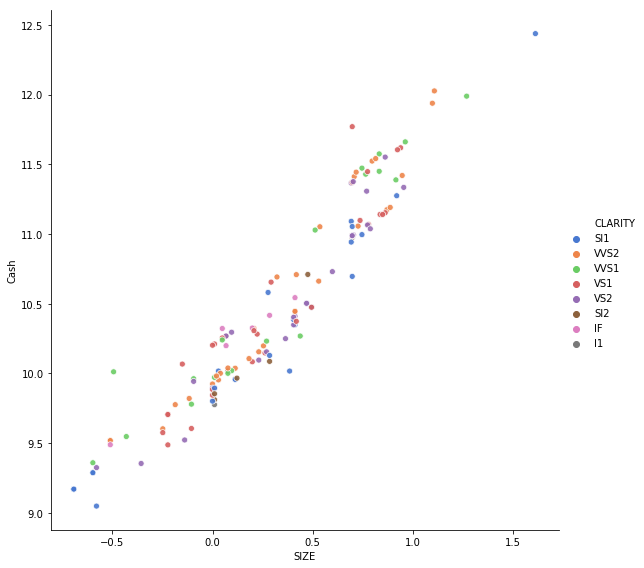
\includegraphics[width=0.45\linewidth]{linear-relation-check-lineplot.png}}
\subcaptionbox{Visualisation that shows the datapoints as a scatterplot along with a linear model fit.\label{fig:linear-relation-check-regplot}}{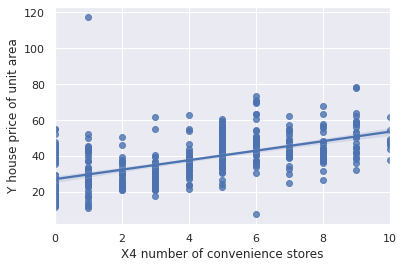
\includegraphics[width=0.45\linewidth]{linear-relation-check-regplot.png}}
\caption{Examples of visualisations used to check linear relationship in data.}
\label{fig:linear-relation-check}
\end{figure*}

Linear machine learning models achieve optimal performance when the target variable can be expressed as a linear combination of the input features. However, features within a dataset that exhibit a linear relationship are considered redundant as they convey the same information to the model during training. Consequently, the feature engineering stage often involves removing such features to create a more efficient training dataset~\ref{shome2022data}. Figure~\ref{fig:linear-relation-check} illustrates two methods for identifying these linear relationships. In Figure~\ref{fig:linear-relation-check-lineplot}, the practitioner assesses the linearity between the features \texttt{Cash} and \texttt{SIZE}. Figure~\ref{fig:linear-relation-check-regplot} depicts the visualization of the feature \texttt{X4} alongside the target variable \texttt{Y}, accompanied by a fitted linear regression model.

\subsubsection{Resource check ($N = 7$)}
% (P71, P86, O64, O66, P68, P82, P107)

\begin{table}
\centering
\caption{Examples of cell outputs used to verify if different types of resources are available on the system where the notebook is being executed.}
\begin{tabular}{@{}m{0.1\textwidth} m{0.05\textwidth} m{0.4\textwidth} m{0.3\textwidth}@{}}
\toprule
\emph{\textbf{Type of resource}}&
\emph{\textbf{Key}}&
\emph{\textbf{Code}}&
\emph{\textbf{Description}}\\
\midrule

External library&
P71&
\begin{lstlisting}
print('Hub version: ', hub.__version__)
\end{lstlisting}&
Check the version of an external Python library installed on the current system.\\

Compute resources&
P68&
\begin{lstlisting}
print('GPU is available')
\end{lstlisting}&
Check if a GPU is available on the current system.\\

Data or pre-trained models&
O66&
\begin{lstlisting}
prostate_cancer_df.shape
\end{lstlisting}&
Check that the dataset has been loaded into memory.\\
\bottomrule
\end{tabular}
\label{tab:resource-check}
\end{table}

\todo{perhaps also add the keys of the case-studies here?}
Table~\ref{tab:resource-check} presents case studies where the output is used to verify that certain resources are available on the system in which the notebook is being executed. We find checks for the availability of compute resources (such as a GPU or a TPU), checking that the dataset or a pre-trained model has been loaded correctly and checks to ensure that a certain version of an external library is present on the system.

P71 highlights the lack of proper software engineering best practices within Jupyter notebooks. This shortcoming in computational notebooks has been identified by prior studies~\cite{quaranta2021kgtorrent, pimentel2019large-scale}. In this case study, managing dependencies through external tools is recommended. Python's built-in \emph{requirements.txt}~\footnote{https://pip.pypa.io/en/stable/reference/requirements-file-format/} file allows specifying dependencies and versions. Alternatively, external programs like \emph{pipenv}~\footnote{https://pipenv.pypa.io/en/latest/} and \emph{poetry}~\footnote{https://python-poetry.org/} use lockfiles to ensure specific version control, guaranteeing reproducibility across different systems. 

\subsubsection{Execution time check ($N = 1$)}
% (P66)

\begin{lstlisting}
print('Total Run Time:')
\end{lstlisting}

While training multiple machine learning models for a single task is common, choosing the best model considers not only its performance but also its training speed. Faster training times are more cost-effective for iterative tasks and promote sustainability in the long run. The provided code snippet (Listing~\ref{lst:exec-time-check}) exemplifies this concept by showcasing a case study (P66) that tracks training times for various models using a grid search. This approach allows practitioners to compare model performance alongside training efficiency. 

\subsubsection{Missing value check ($N = 3$)}
% (O12, O36, P74)

Checking for missing values is a critical step in the preprocessing phase of a machine learning project because it significantly influences the quality and performance of the model. Missing data can lead to biased or incorrect conclusions if not handled properly, potentially skewing the model's performance by training on incomplete or non-representative samples~\cite{shome2022data}. Many machine learning algorithms, including those that involve matrix multiplication operations such as linear regression and neural networks, demand complete numerical datasets to perform calculations. Missing values interrupt these calculations, leading to errors or the inability to execute algorithms entirely.

\begin{table}
\centering
\caption{Examples of cell outputs used to check for missing data.}
\begin{tabular}{@{}m{0.05\textwidth} m{0.6\textwidth}@{}}
\toprule
\emph{\textbf{Key}}&
\emph{\textbf{Code}}\\
\midrule

P74&
\begin{lstlisting}
print(train_df.isnull().sum())
\end{lstlisting}\\

O12&
\begin{lstlisting}
sns.heatmap(test_df.isnull(), yticklabels=False, cbar=False, cmap='viridis')
\end{lstlisting}\\

O36&
\begin{lstlisting}
test.isna().sum().unique()
\end{lstlisting}\\
\end{tabular}
\label{tab:missing-value}
\end{table}

Table~\ref{tab:missing-value} presents all case studies where cell outputs were used to check for missing data. While \emph{P74} and \emph{O36} perform this check in code, \emph{O12} presents a visual representation of missing data using a heatmap.

\subsubsection{Model performance check ($N = 33$)}
% (O3, O50, O52, O57, O74, P3, P6, P8--12, P16--19, P23, P24, P28, P30, P34, P42, P47, P48, P50, P51, P54, P55, P57, P58, P61, P78, P93)

\begin{table}
\centering
\caption{Various cell outputs used to check the performance of an ML model after training.}
\begin{tabular}{@{}m{0.05\textwidth} m{0.6\textwidth}@{}}
\toprule
\emph{\textbf{Key}}&
\emph{\textbf{Code}}\\
\midrule

P3&
\begin{lstlisting}
print('The mean accuracy with 10 fold cross validation is: %s ' % round(scores * 100, 2), '%')
\end{lstlisting}\\
    
P6&
\begin{lstlisting}
print('RMSE:', np.sqrt(metrics.mean_squared_error(y_test, pred)))
\end{lstlisting}\\

P18&
\begin{lstlisting}
print('The Accuracy is:', accuracy_score(y_test, y_pred))
\end{lstlisting}\\

P18&
\begin{lstlisting}
print('Classification Report: SVM (validation data)')
\end{lstlisting}\\

P54&
\begin{lstlisting}
print('Intercept value:', lm.intercept_)
\end{lstlisting}\\
\end{tabular}
\label{tab:model-perf}
\end{table}

The performance is printed to compare against other models/variations in the experimental model development phase; during the continuous experimentation phase, the author might change parameters of the model or change the data (engineer features, etc) and then re-run the model to check if the performance improved

Table~\ref{tab:model-perf} presents a few examples of cell outputs used to check the performance of a trained ML model. Besides \emph{accuracy}, we also see checks for the \emph{Root Mean Square Error (RMSE)} and the use of the classification report provided by scikit-learn~\footnote{https://scikit-learn.org/stable/modules/generated/sklearn.metrics.classification\_report.html}. In addition to the accuracy, the classification report also reports the \emph{precision}, \emph{recall} and \emph{f1 score} for all labels present in the target feature.

\emph{P54} prints the intercepts of a linear regression model. Checking the intercept of a linear regression model is essential for understanding the baseline prediction when all predictors are zero, interpreting the model, identifying potential data biases or missing variables, assessing model validity, and comparing baseline predictions across different models. This insight is critical for accurate model interpretation and effective decision-making in practical applications.

\begin{wrapfigure}{l}{0.45\linewidth}
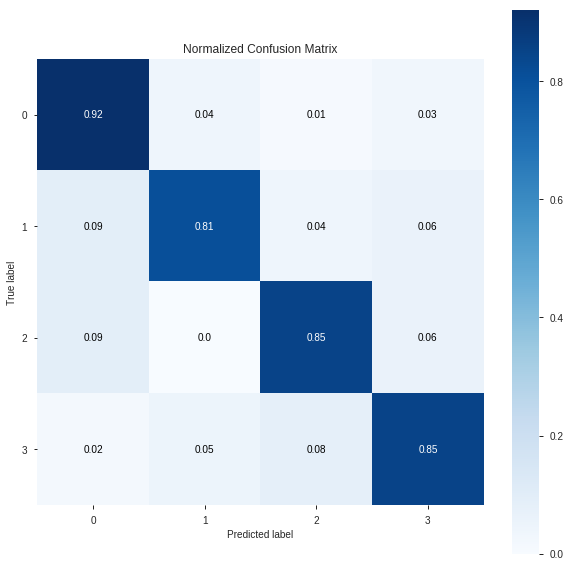
\includegraphics[width=\linewidth]{model-perf-confusion-matrix.png}
\caption{Confusion matrix}
\label{fig:model-perf-confusion-matrix}
\end{wrapfigure}

Figure~\ref{fig:model-perf-confusion-matrix} shows a heatmap used to visualise the confusion matrix of a multi-label classification task. The values are normalised using the actual number of examples of each class which makes the comparisons of the values across the classes possible.

% TODO: this looks horrible if we are wrapping text around the figure above
% \begin{lstlisting}[caption={Spot-check the performance of an image classification model for a random sample of input images.}, label={lst:model-perf-custom}]
% def spot_check_recs(classifier, seed):
%     random_images = []
%     random_labels = []
%     random_loc = np.random.randint(3000)
%     distance, loc = classifier.kneighbors( embedding_model.predict( visualize[random_loc].reshape(-1,28,28)), 100)
    
%     random_images.append(visualize[random_loc])
%     ...
%     for rec_loc, dist in zip(loc.reshape(-1,1), distance.reshape(-1,1)):
%         ...
        
%     ImageUtil.grid_display(random_images, random_labels, no_of_columns=1, figsize=(2,2), fig_title = "recs")

% spot_check_recs(classifier, 910)
% \end{lstlisting}

% Listing~\ref{model-perf-custom} shows a function implemented by a practitioners to manually evaluate an image classification model on a random sample of input images. The function prints the input image along with the prediction of the model which the practitioner uses to spot-check the performance of the model.

\subsubsection{Neural network architecture ($N = 1$)}
% (P92)

\begin{lstlisting}[caption={Print the architecture of a neural network.}, label={lst:network-architecture}]
print(MyNetwork)
\end{lstlisting}

Listing~\ref{lst:network-architecture} shows a print statement to show the architecture of a neural network. Printing the structure of a neural network serves crucial purposes such as verifying the correct implementation of the architecture, aiding in debugging by ensuring layer compatibility, and providing a clear, human-readable format for documentation and educational insights. It helps in verifying configurations like layer dimensions and operations before initiating computationally intensive training, ensuring the model is set up efficiently for the intended tasks. This practice is fundamental for maintaining accuracy, facilitating collaboration, and enhancing the reproducibility of the model.

\subsubsection{Shape check ($N = 3$}
% (P4, P32, P117)

Ensuring that data dimensions align with expectations is important particularly following data pre-processing or transformation steps.

Primarily, the number of features in the training set must match those in the testing set. This alignment is crucial because statistical machine learning models are trained on specific data dimensions and expect the same dimensional structure during inference to perform accurately. Similarly, in neural network architectures, the configuration of input layers depends directly on the shape of the training data, dictating the number of input neurons needed. Furthermore, the correspondence between the number of test examples and their respective labels is essential for accurately computing performance metrics, such as accuracy.

\begin{table}
\centering
\begin{tabular}{@{}m{0.05\textwidth} m{0.8\textwidth}@{}}
\toprule
\emph{\textbf{Key}} & \emph{\textbf{Code}}\\
\midrule
P4 &
\begin{lstlisting}
print('no.of examples in test data : ', len(test_data))
\end{lstlisting}\\
P32 &
\begin{lstlisting}
print('Training set shape : ', x_train.shape) 
\end{lstlisting}\\
\end{tabular}
\caption{Example of outputs used to check the shape of the data.}
\label{tab:shape-check}
\end{table}

Table~\ref{tab:shape-check} shows two print statements discovered in this study which demonstrate routine checks performed by developers to ensure the integrity and applicability of their models. Such checks are indicative of the meticulous attention to detail necessary in the model training and validation process, underscoring the importance of shape validation in achieving reliable machine learning outcomes.

\subsubsection{Type check ($N = 2$)}
% (O71, P43)

Ensuring data types align with model requirements is a fundamental step in the exploratory data analysis (EDA) phase of developing machine learning models. Since all machine learning algorithms perform mathematical operations, such as matrix multiplications, they require the input data to be entirely numerical to avoid computational errors. The process of checking data types helps in identifying the necessary pre-processing or transformation steps to convert the data into a form that is compatible with these models. For example, while numerical features often require normalisation to bring them within a specific scale, categorical features must be converted into a numerical format through methods like one-hot encoding to ensure they can be effectively integrated into the model.

This is illustrated in our analysis, where checks such as \texttt{print('data type:', images.dtype)} and \texttt{type(Y)} are employed to verify the data types of variables. These type checks are crucial not only for confirming the current state of the data but also for determining the specific transformations required to make the data suitable for subsequent modelling steps.

This proactive approach in the EDA phase facilitates smoother transitions into model training and can significantly impact the performance and effectiveness of the final machine learning models.

\subsubsection{Value check/ Spot checks ($N = 5$)}
% (O56, O60, P64, P67, P114)

\begin{table}
\centering
\begin{tabular}{@{}m{0.05\textwidth} m{0.8\textwidth}@{}}
\toprule
\emph{\textbf{Key}}&
\emph{\textbf{Code}}\\
\midrule

O60 &
\begin{lstlisting}
X_pca.head()
\end{lstlisting}\\
\end{tabular}
\caption{Example of outputs used to perform spot checks.}
\label{tab:shape-check}
\end{table}

Table~\ref{tab:spot-check} presents outputs which were used to spot check at various stages of the ML development cycle. Performing value or spot checks can be an essential practice for ensuring data integrity and model accuracy at various stages of development. These checks are crucial for verifying that operations such as data transformations, model predictions, and feature engineering are functioning as expected.

In \emph{O60}, the analyst verifies that the number of features in the data matches expectations after apply Principal Component Analysis (PCA). This is a critical step for maintaining dimensional consistency in feature-reduced datasets.

% In another case, P64, which is particularly relevant in image processing contexts, the maximum value in the second channel of a 3D numpy array is extracted and verified using np.max(cur[:, :, 1]), ensuring that the data manipulation retains its expected properties.

% The check in P67 involves a manual verification of the output of an activation function in a neural network, which is essential for confirming the functional efficacy of neural components in model training. 

% Lastly, P114 assesses the correctness of one-hot encoding, a fundamental preprocessing step for categorical data, ensuring that the transformation has been executed correctly as seen with print(onehot_encoded). Each of these checks not only validates individual transformations or predictions but also reinforces the overall reliability and robustness of the machine learning models being developed.

\subsubsection{Model training (O8, O31, O42, P77)}

O8, P77: Periodically print the progress made in training by printing the training loss/accuracy of model.

O31: check the model fits the data without any errors; this is done in the model experimentation phase, where several models are tested and the best one based on the selection criteria is picked

\subsection{Explicit feedback using \texttt{assert} statements}

% TODO: bring in the notion of pre and post condition checks (the wikipedia page on assertions is very interesting: https://en.wikipedia.org/wiki/Assertion_(software_development)); specifically the part on run-time assertions

\todo{TODO: find out more about batch training}
\subsubsection{Batch size check (A21, A28, A70)}

Neural Networks are trained using smaller batches that makes it more efficient use of hardware GPU cores. During batch training the weights are not updated with every example but with the average of the entire batch, this ensures a more optimal and smoother learning curve and generally leads to better generalizability.

When trained using batches, we need to take this into account when calculating the performance of the model. We need to calculate the accuracy over multiple batches and then average the results.

We encounter assertions that check the size of the batch prior to training. This is to ensure that the batch size matches the hardware specifications? We should not have a batch size that does not fit in the memory of GPU/CPU.


\subsubsection{Data leakage check (A33)}

It is a best practise to ensure that the ML model is not tested using examples that it has already encountered during training. This is to ensure that the model is not overfitting on the training data and is able to generalise to examples similar to the distribution of the training set, but not exactly the same. In A33 we see that the assert ensures that the training and validation sets do not share any examples.

\subsubsection{Dependency check (A18, A67)}
\todo{TODO: what is the motivation of this assertion? Find prior work on python dependency management?}

This is a unique type of test which occurs due to the unique workflow of notebooks. Typically dependencies are managed through external means such as dedicated dependency management solutions or the builtin Python method using a requirements.txt file. We notice assertions that check that the major version of an external dependency is equal to the specified value.

\todo{NOTE: missing-value-check and existence-check}

\subsubsection{Existence check (A86)}

Existence checks are carried out in various contexts. Most are for checking that columns in a dataset do not contain missing values. Others ensure that certain columns (such as the column containing the labels of the data) exists in the dataset prior to splitting the data into training and testing sets. Existence checks are frequently performed after data pro-processing  steps are performed to ensure that missing values were not added to the dataset.

\todo{TODO: we need to elaborate this one with examples}

\subsubsection{Mathematical property checks (A3, A25, A56, A64)}

Machine learning models are often rooted in statistical models. Implementing neural networks requires a grasp of linear algebra and matrix multiplication. We find several assertions that test the mathematical properties of arrays and matrices after performing matrix operations.

\subsubsection{Model performance check (A7, A15, A19, A22, A24, A26, A38, A54, A58, A59, A72)}

We see several assertions that test for the performance of the trained ML model against a validation or test test. The assertions often compare a performance metric (such as accuracy, precision, recall, F1, etc) against a predefined threshold.

\todo{TODO: this needs more work and investigation}
\subsubsection{Network architecture check (A11)}

We only have one example here.

% TODO lots to elaborate and discuss here
\subsubsection{Resource check (A10, A14, A37, A60, A74)}

We find assertions that check that a pre-trained model exists on the file system, or that data can be loaded from a specified file path. There are also checks that ensure that a visualisation created using matplotlib contains data in it.

\subsubsection{Data shape check (A5, A9, A13, A16, A17, A29, A31, A61, A71, A76--78, A82, A84, A85, A89, A90, A91, A93--96, A98--101)}

``Swiss army knife'' of assertions!

\subsubsection{Type check (A2, A35, A40, A81, A88)}

Checking the data type of features and such.

\subsubsection{Value check (A30, A41, A44--46, A52, A65, A68, A69, A73, A92)}

Check that the values in a column are in the specified values (categorical) or in a specified range (normalised continuous variable) or binary (such as the label column).

% NOTE: blanks and unit-tests
\subsubsection{Miscellaneous checks (A6, A20, A32, A34, A36, A53, A62, A75, A83, A87, A97)}

These feel like unit tests, performed in lieu of writing full test suites in the notebook.

%\begin{acknowledgements}
%If you'd like to thank anyone, place your comments here
%and remove the percent signs.
%\end{acknowledgements}


% Authors must disclose all relationships or interests that 
% could have direct or potential influence or impart bias on 
% the work: 
%
% \section*{Conflict of interest}
%
% The authors declare that they have no conflict of interest.


% BibTeX users please use one of
% \bibliographystyle{spbasic}      % basic style, author-year citations
\bibliographystyle{spmpsci}      % mathematics and physical sciences
%\bibliographystyle{spphys}       % APS-like style for physics
\bibliography{bibliography}   % name your BibTeX data base

\subsection{Assertions derived from visualisations}
\end{document}
% end of file template.tex

